\documentclass[portrait,a0,final]{a0poster}

\usepackage[a0paper,pass]{geometry}

\usepackage{amsmath}
\usepackage{mathtools}

\usepackage{bm}
\usepackage{scalerel}
\usepackage{helvet}
\usepackage{textcomp}
\usepackage{fontenc}
\usepackage{anyfontsize}
\usepackage{microtype}
\usepackage{shadowtext}
\usepackage[british]{babel}
\usepackage{blindtext}

\usepackage{sectsty}
\sectionfont{\fontsize{40}{40}\selectfont}

\usepackage{ifthen}

\usepackage[cmyk]{xcolor}
\usepackage{tikz}
\usepackage{graphicx}

\hyphenation{Although}
\hyphenation{consideration}
\hyphenation{hyperparameters}
\hyphenation{learning}

\usetikzlibrary{shapes,fadings,calc,decorations.pathmorphing,arrows}

\renewcommand\familydefault{\sfdefault}

\definecolor{tudblue}{cmyk}{1,0,0,0}
\definecolor{barcolor}{hsb}{0.56, 0.40, 1}
\definecolor{arrowcolor}{hsb}{0.56, 0.20, 1}

\begin{document}
\thispagestyle{empty}
\def\mytitle{}
\begin{tikzpicture}[remember picture, overlay, shift={(current page.south west)}, every node/.style={inner sep=0}]

%%%%	Header coordinates.
\coordinate (header_SW)      at (              0 , 0.9\paperheight  );
\coordinate (header_NE)      at ( 1.1\paperwidth , 1\paperheight  );
\coordinate (header_fade_SW) at (              0 , 0.805\paperheight  );
\coordinate (header_fade_NE) at ( 1.1\paperwidth , 0.901\paperheight );
\coordinate (title)          at ( 0.5\paperwidth , 0.935\paperheight );
\coordinate (authors)        at ( 0.5\paperwidth , 0.865\paperheight );
\coordinate (institute)      at ( 0.5\paperwidth , 0.835\paperheight );

%%%%	Footer coordinates.
\coordinate (footer_SW)  at (              0 , 0                 );
\coordinate (footer_NE)  at ( 1.1\paperwidth , 0.05\paperheight );
\coordinate (tudlogo_SW) at (0.01\paperheight, 0.01\paperheight  );
\coordinate (tudlogo_SE) at (0.1325\paperwidth, 0.009\paperheight  );
\coordinate (faculty_W) at (0.56\paperwidth, 0.015\paperheight  );
\def\tudlogoheight{0.03\paperheight}

%%%%	Header: Cyan banner fading south, with title and 
\fill[tudblue] (header_SW) rectangle (header_NE);
\fill[tudblue] (header_fade_SW) rectangle (header_fade_NE);
\node at (title) [anchor=center] {\parbox{0.9\paperwidth}{\centering\fontsize{95}{120}\bfseries\color{white}\shadowoffset{2pt}\shadowcolor{black!55!white} \shadowtext{Learning and Optimizing Probabilistic Models}\\\shadowtext{for Planning under Uncertainty}}};
\node at (authors) [anchor=center] {\parbox{0.9\paperwidth}{\centering\fontsize{60}{60}\selectfont\color{white} \shadowtext{R. van Bekkum,}\hskip1.5em \shadowtext{M. T. J. Spaan}}};
\node at (institute) [anchor=center] {\parbox{0.9\paperwidth}{\centering\fontsize{45}{45}\selectfont\color{white} \shadowtext{Algorithmics Group, Department of Software Technology}}};

%%%%	Footer: Cyan banner with logo embedded.
\fill [tudblue] (footer_SW) rectangle (footer_NE);
\node at (tudlogo_SW) [anchor=south west] {\includegraphics[height=\tudlogoheight ]{figures/TU_Delft_logo_White}};
\node at (tudlogo_SE) [anchor=south west] [white,text width=0.2\paperwidth] {\fontsize{18}{19}\selectfont Delft\\University\hskip0.175cmof\\\hskip0.0275cm Technology\\};

\node at (faculty_W) [anchor=west] [white] {\parbox{0.6\paperwidth}{\Large\bfseries Electrical Engineering, Mathematics, and Computer Science}};

%%%%	Contents coordinates
\coordinate (abstract) at (0.045\paperwidth, 0.7 \paperheight);
\coordinate (baseframework) at (0.045\paperwidth, 0.515 \paperheight);
\coordinate (multiframework) at (0.045\paperwidth, 0.275\paperheight);
\coordinate (experiments) at (0.505\paperwidth, 0.53\paperheight);
\coordinate (conclusions) at (0.505\paperwidth, 0.194\paperheight);

%%%%	Contents
\node at (abstract) [anchor=west, black, text width=0.4\paperwidth] {

\parbox{\textwidth}{
\section*{Abstract}
Decision-theoretic planning techniques are increasingly being used to obtain (optimal) plans for domains involving uncertainty, which may be present in the form of the controlling agent's actions, its percepts, or exogenous factors in the domain.
These techniques build on detailed probabilistic models of the underlying system, for which Markov Decision Processes (MDPs) have become the \textit{de facto} standard formalism.
However, handcrafting these probabilistic models is usually a daunting and error-prone task, requiring expert knowledge on the domain under consideration.
Therefore, it is desirable to automate the process of obtaining these models by means of learning algorithms presented with a set of execution traces from the system.
Although some work has already been done on crafting such learning algorithms, the state of the art lacks an automated method of configuring their hyperparameters, so to maximize the performance yielded from executing the derived plans.

\bigskip

In this work we present a solution that employs the \textit{Bayesian Optimization} (BO) framework to learn MDPs autonomously from a set of execution traces, optimizing the expected value and performance in simulations over a set of tasks the underlying system is expected to perform.
The approach has been tested on learning MDPs for mobile~robot navigation, motivated by the significant uncertainty accompanying the robots' actions in this domain.
}
};

\node at (baseframework) [anchor=west, black, text width=0.4\paperwidth] {
	
\parbox{\textwidth}{
\section{Base Framework}
In our solution we employ BO to select hyperparameters $\theta$ for model learning algorithms towards a global maximizer of a performance measure $V_\mathcal{M}$ (made through time-expensive simulations) over a set of tasks the system is expected to perform.

\bigskip\bigskip

\includegraphics[width=\textwidth]{figures/learning-cycle-simplified}
}
};

\node at (multiframework) [anchor=west, black, text width=0.4\paperwidth] {
	
%\parbox{\textwidth}{
\section{Multi-Phase Framework}
To improve the cost-effectiveness, the solution is extended by defining two phases. In the first phase an optimization is done on a relatively cost-cheap performance measure based on the value functions computed from the learned MDPs.
The resulting posterior is used to potentially speed up the optimization in the second phase by steering the BO acquisition of new samples.

\bigskip
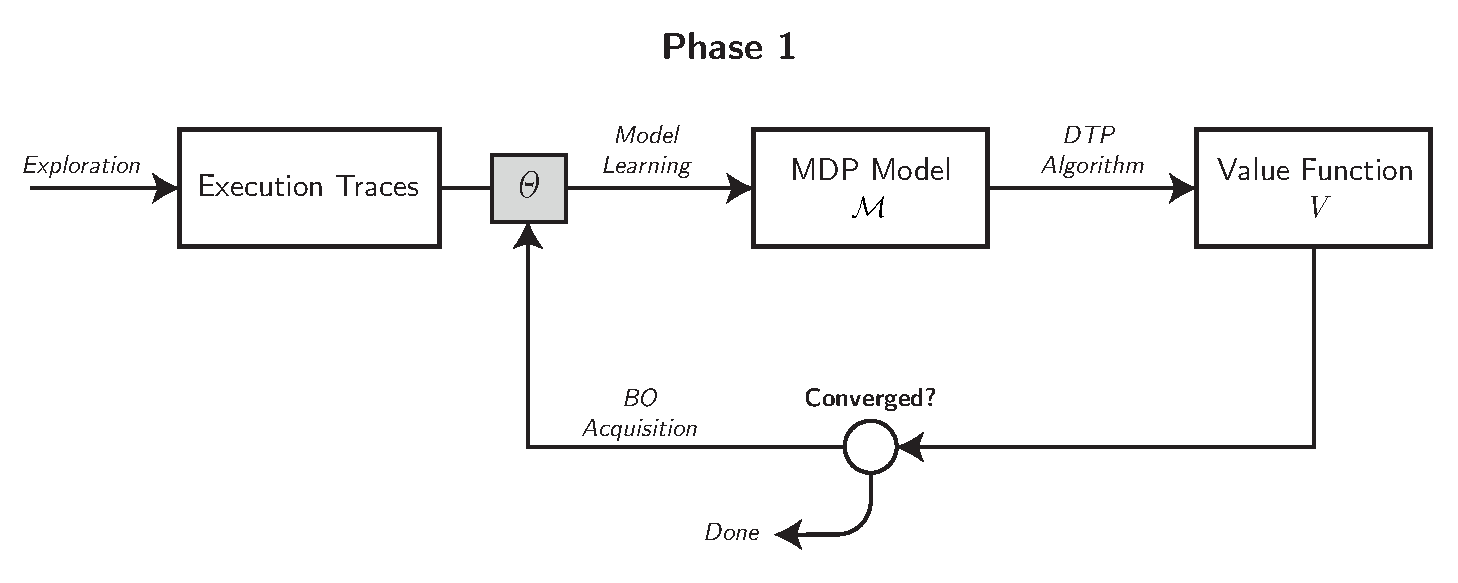
\includegraphics[width=\textwidth]{figures/phase-1}

\vspace{2cm}

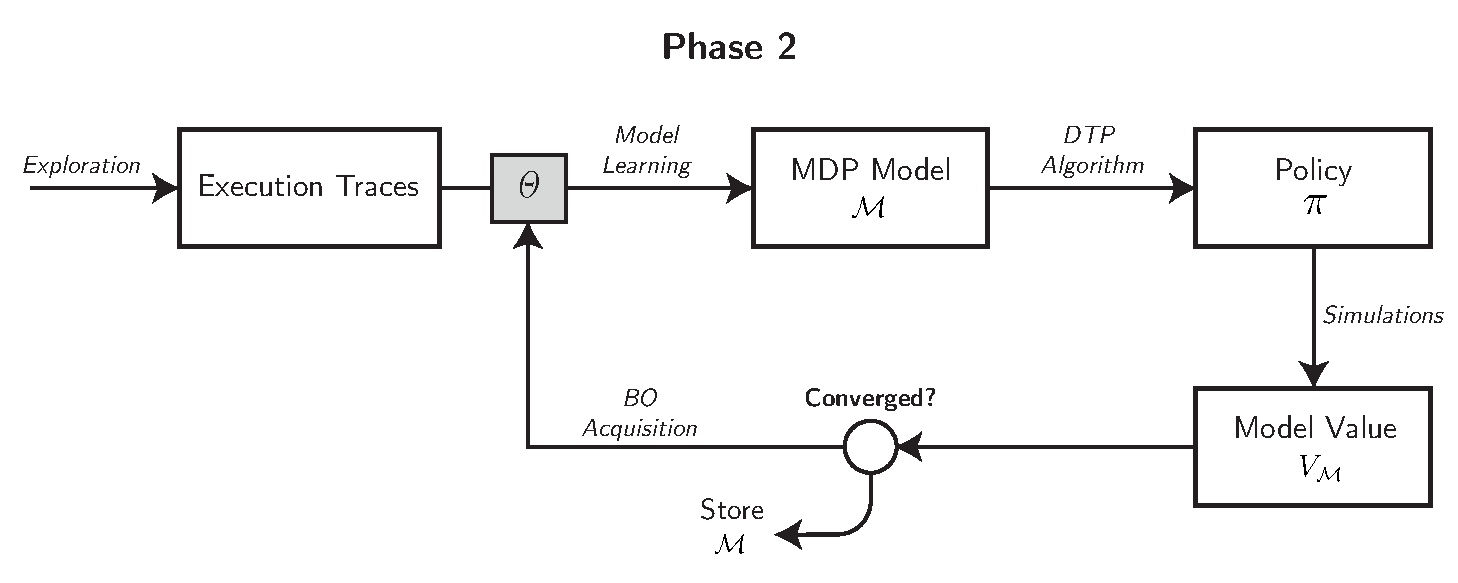
\includegraphics[width=\textwidth]{figures/phase-2}
%}
};


\node at (experiments) [anchor=west, black, text width=0.45\paperwidth] {
	
\parbox{\textwidth}{
\section{Experimental Setup and Results}
For our experiments an implementation has been made for path planning in mobile robot navigation, where a mobile robot is controlled by learned MDPs in simulation environments inside the \textit{Morse} robotics simulator. Based on execution traces from a random action policy, MDPs are learned based on clustering and maximum likelihood algorithms.

\bigskip

\begin{minipage}{\textwidth}
\centering
\raisebox{-0.5\height}{\includegraphics[width=0.475\textwidth]{figures/demo_clustering_2}}
\hspace*{1em}
\raisebox{-0.5\height}{\includegraphics[width=0.475\textwidth]{figures/demo_trajectory}}
\end{minipage}

\bigskip

The plots below show the resulting GP posteriors for a selection of our experiments, from which we can identify the hyperparameters $\theta$ most likely to maximize the system's performance.

\vspace{2.5cm}

\begin{center}
\large \textsf{BASE FRAMEWORK}
\end{center}

\vspace{1cm}

\begin{minipage}{\textwidth}
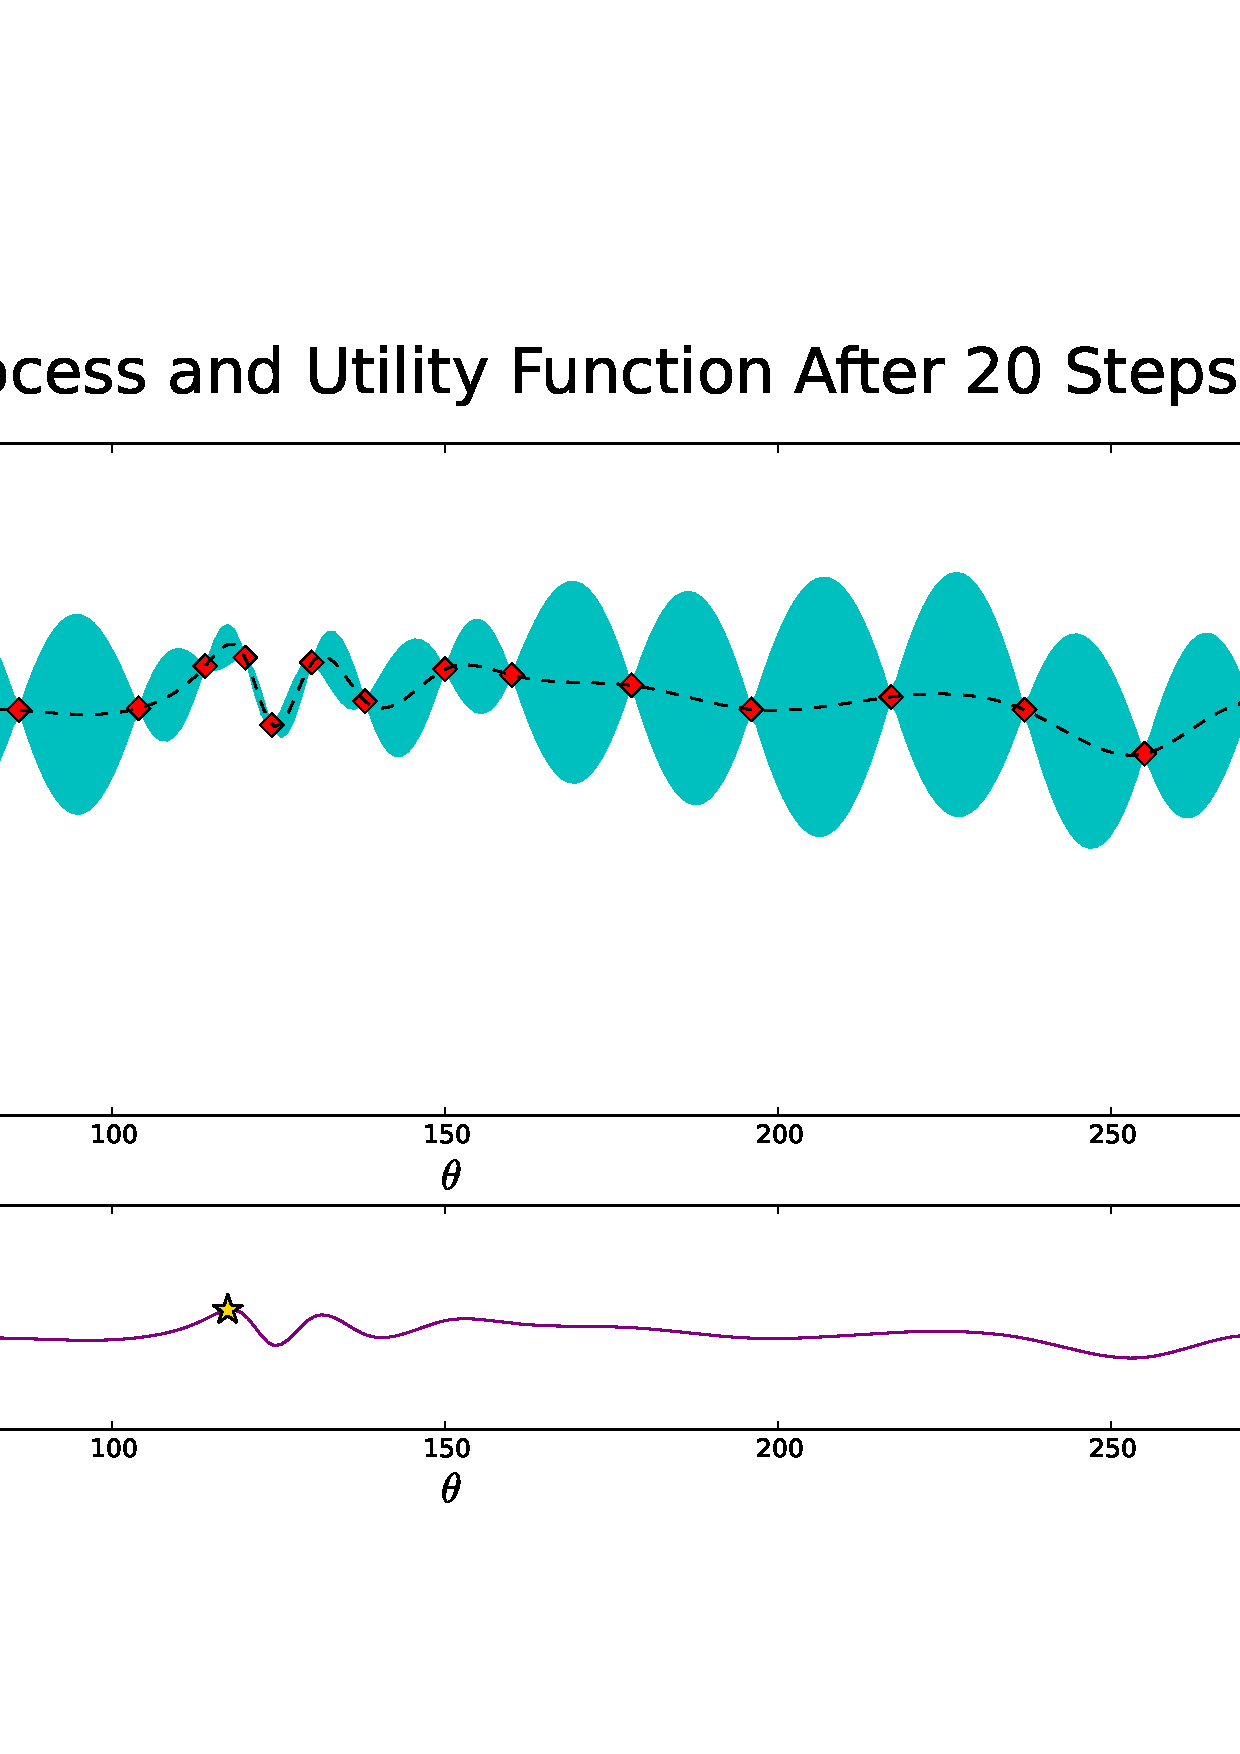
\includegraphics[width=0.5\textwidth]{../figures/plots/tum_base/plot_b_00__alg_kmeans_pct_100_acq_ei.pdf}
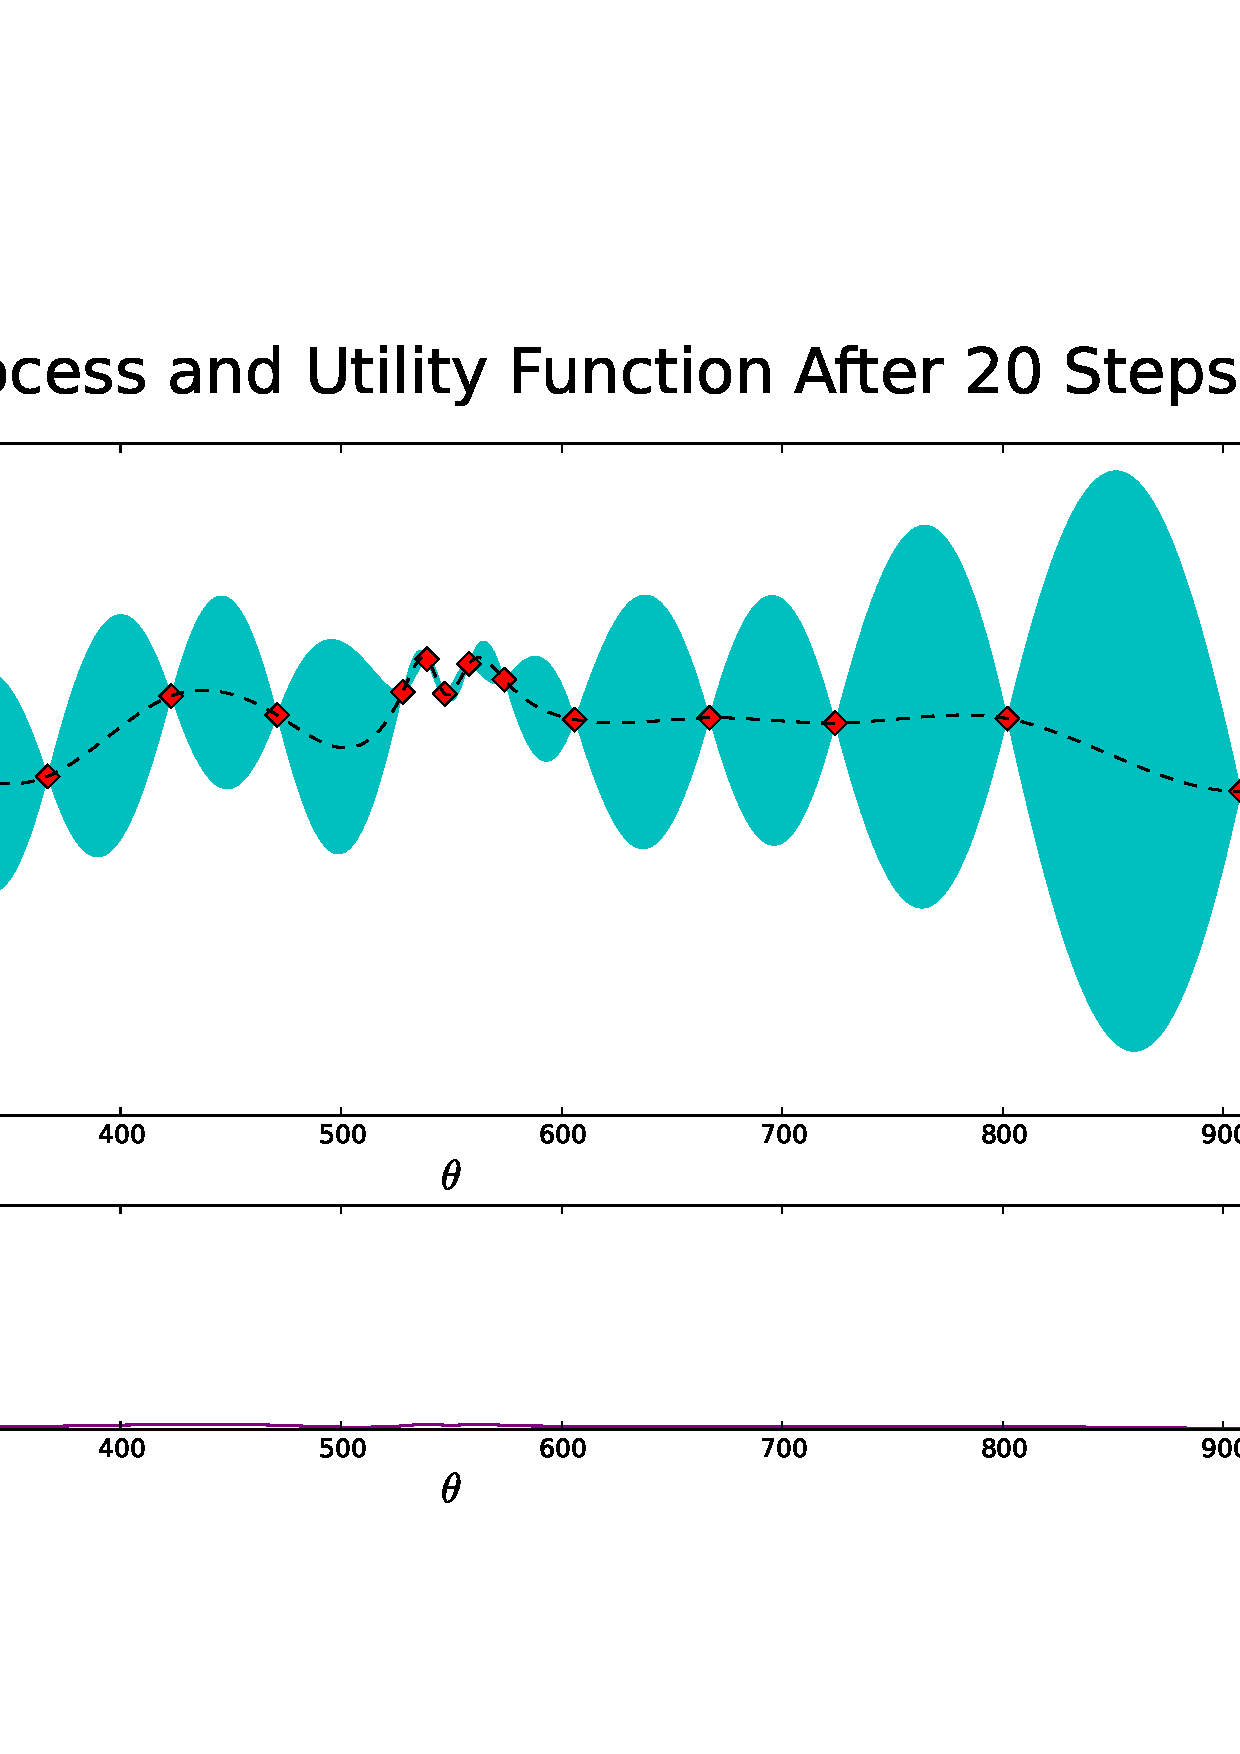
\includegraphics[width=0.5\textwidth]{../figures/plots/uol_base/plot_b_00__alg_kmeans_pct_100_acq_eips.pdf}
\begin{minipage}{0.5\textwidth}
\centering
\small
\texttt{tum\_kitchen} environment, \textrm{EI} acquisition function
\end{minipage}
\begin{minipage}{0.5\textwidth}
\centering
\small
\texttt{uol\_bl} environment, \textrm{EIPS} acquisition function
\end{minipage}
\end{minipage}

\vspace{3cm}

\begin{center}
\large \textsf{MULTI-PHASE FRAMEWORK}
\end{center}

\vspace{1cm}

\begin{minipage}{\textwidth}
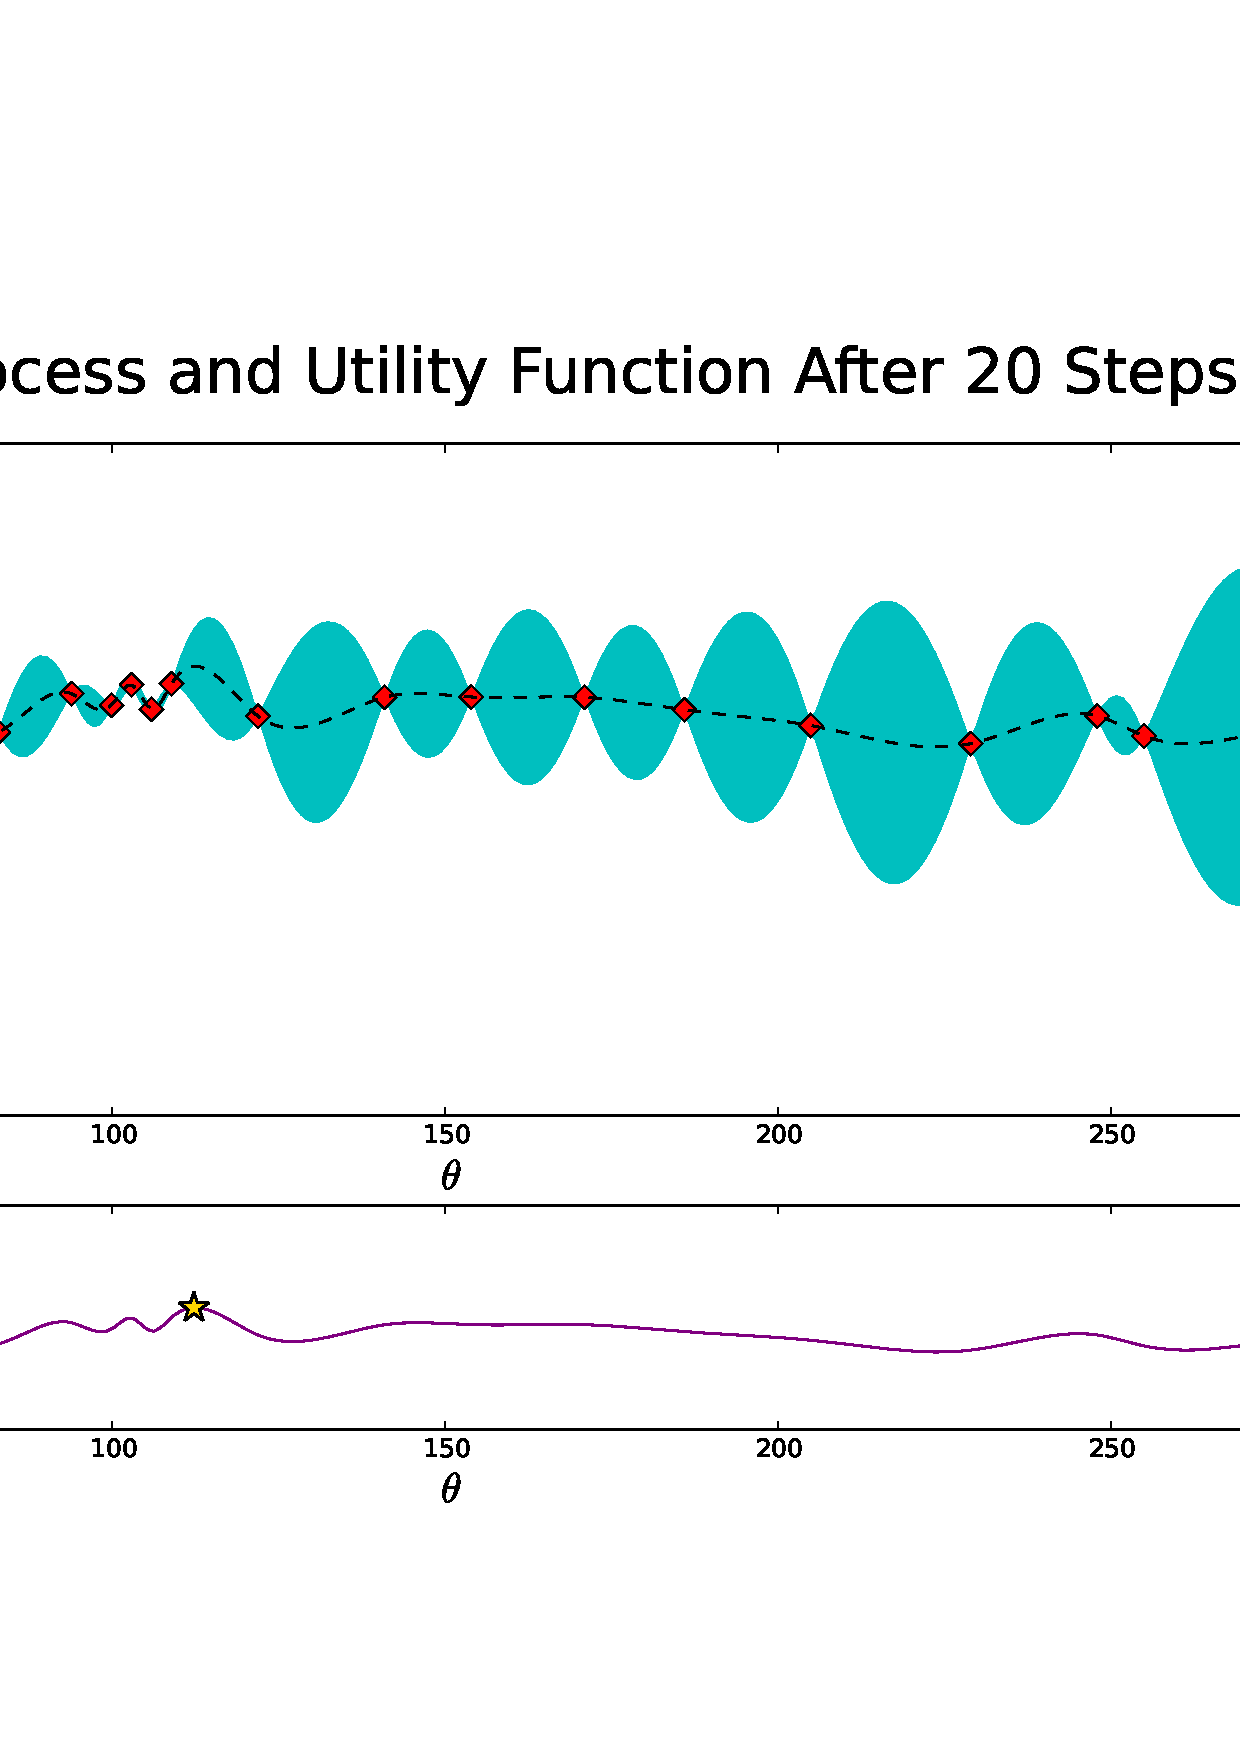
\includegraphics[width=0.5\textwidth]{../figures/plots/tum_multi/plot_b_00__alg_kmeans_pct_100_acq_ei.pdf}
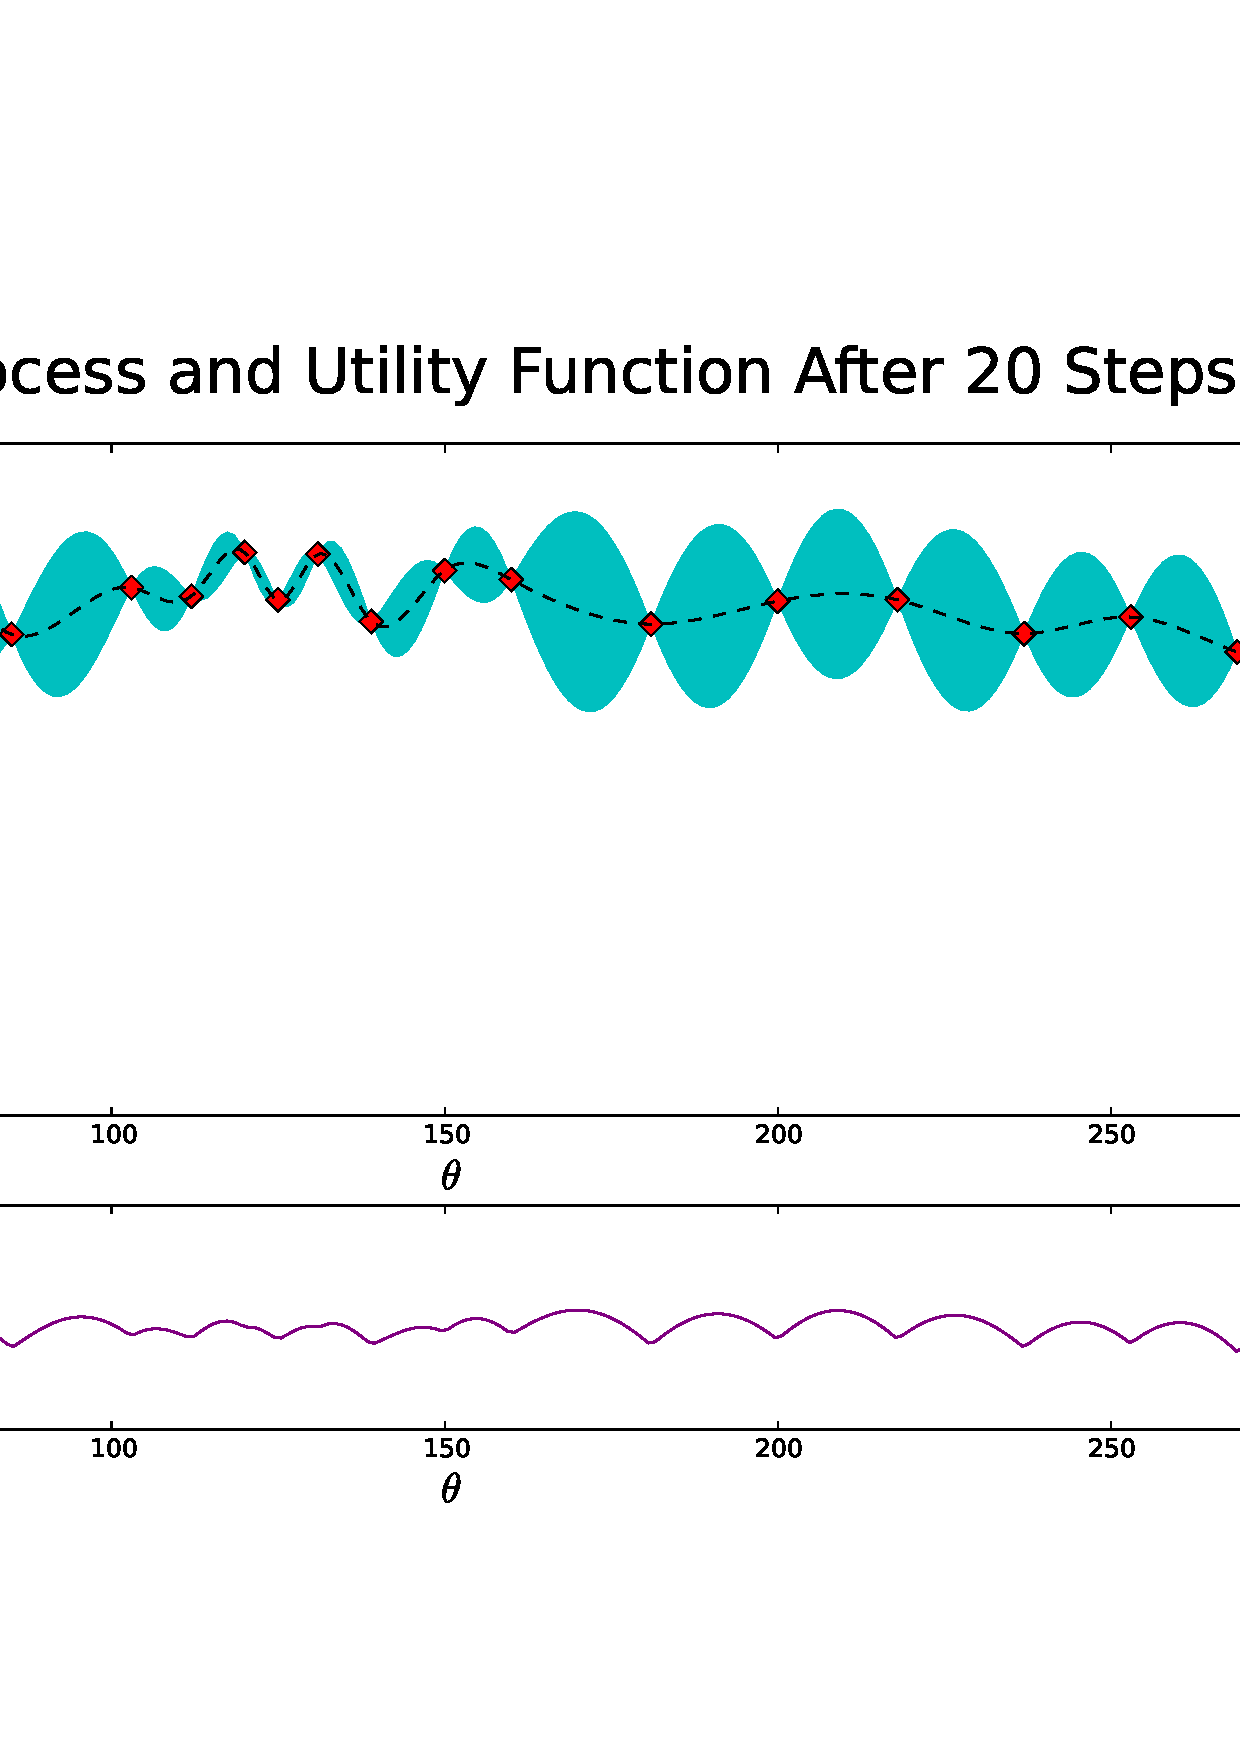
\includegraphics[width=0.5\textwidth]{../figures/plots/uol_multi/plot_b_00__alg_kmeans_pct_100_acq_ucb.pdf}
\begin{minipage}{0.5\textwidth}
\centering
\small
\texttt{tum\_kitchen} environment, \textrm{EI} acquisition function
\end{minipage}
\begin{minipage}{0.5\textwidth}
\centering
\small
\texttt{uol\_bl} environment, \textrm{GP-UCB} acquisition function
\end{minipage}
\end{minipage}

}
};

\node at (conclusions) [anchor=west, black, text width=0.45\paperwidth] {
	
	\parbox{\textwidth}{

\section{Conclusions}
As handcrafting MDPs for systems with uncertain dynamics is a difficult task, an appealing approach is to automate the task by employing learning algorithms on a dataset describing the dynamics of the underlying system.
Evaluating all hyperparameter settings for these algorithms is a cost-expensive endeavour which may be more effectively approached by BO.
Our multi-phase approach may speed up the optimization making relatively cost-cheap performance assessments on a more abstract level first, and using these to steer the acquisition in an optimization where more accurate and cost-expensive performance assessments are made through simulations or execution in a real-world setting.
}
};

\end{tikzpicture}

\end{document}
